% wfbook
% wfbook.tex

\documentclass[12pt,UTF8]{ctexbook}

% 设置纸张信息。
\usepackage[a4paper,twoside]{geometry}
\geometry{
	left=25mm,
	right=25mm,
	bottom=25.4mm,
	bindingoffset=10mm
}

\usepackage{graphicx}

% 设置字体,并解决显示难检字问题。
\xeCJKsetup{AutoFallBack=true}
\setCJKmainfont{SimSun}[BoldFont=SimHei, ItalicFont=KaiTi, FallBack=SimSun-ExtB]

% 目录 chapter 级别加点(.)。
\usepackage{titletoc}
\titlecontents{chapter}[0pt]{\vspace{3mm}\bf\addvspace{2pt}\filright}{\contentspush{\thecontentslabel\hspace{0.8em}}}{}{\titlerule*[8pt]{.}\contentspage}

% 设置 part 和 chapter 标题格式。
\ctexset{
	part/name= {第,卷},
	part/number={\chinese{part}},
	chapter/name={第,篇},
	chapter/number={\chinese{chapter}}
}

% 设置署名格式。
\newenvironment{shuming}{\hfill\bfseries\zihao{4}}

% 注脚每页重新编号,避免编号过大。
\usepackage[perpage]{footmisc}

\title{\heiti\zihao{0} wfbook}
\author{WangFei}
\date{\today}

\begin{document}

\maketitle
\tableofcontents

\frontmatter

\chapter{前言}



\mainmatter

\chapter{生殖器官}

\section{女性生殖器官}

女性的生殖器官包括外生殖器官和内生殖器官两部分。外生殖器主要是指阴阜、大阴唇、小阴唇、阴蒂、阴道前庭、尿道口、阴道口、处女膜、前庭大腺和前庭球,而内生殖器则包括阴道、子宫、输卵管和卵巢。

\subsection{外生殖器官}

阴阜在耻骨联合前方,由皮膚及很厚的皮下脂肪层构成。到性成熟期常有阴毛,分步呈倒三角形。

外阴靠近兩股内側的一對长圓形隆起的皺襞為大阴唇。大阴唇外面长有阴毛,皮下是脂肪組織、彈性纖維及靜脈叢。生育前大阴唇自然合攏,生育後向阴阜兩側分開。大阴唇内側有一對小阴唇,是一對黏膜皺襞,表面濕潤,有豐富的神經分佈,因而感覺敏銳。

阴蒂位於兩側小阴唇之間的頂端,是一個长圓形的小器官,末端為一個圓頭,內端與一束薄薄的勃起組織相連接。勃起組織有豐富的靜脈叢和神經末梢,是女性最重要的性感區,對其進行愛撫會引起強烈的性反應。

兩側小陰唇之間的凹陷部分是陰道前庭,陰道前庭表面有黏膜遮蓋,前半部有尿道開口,後半部有陰道開口。尿道口是一個形狀不規則的橢圓小孔,尿液從這裏流出。

陰道口被一塊不完全封閉的黏膜所遮蓋,中間是處女膜。處女膜的正反兩面都是濕潤的黏膜,黏膜之間有結締組織、微血管和神經末梢,中間的小孔即處女膜孔,經血即由此流出。處女膜孔的大小和膜的厚薄程度因人而異。處女膜破後,黏膜變成許多小圓球狀物,成為處女膜痕。

陰道口的兩側有前庭大腺(又稱「巴氏腺」),能分泌液體,有滑潤功能。前庭大腺有小蠶豆般大小,性興奮時能分泌黃白色黏液,起滑潤陰道口作用。正常檢查時摸不到此腺體,如有感染時則會腫大。前庭球又稱為「球海綿體」,是一對海綿體組織,位於陰道口兩側,能勃起。

\begin{figure}
	\centering
	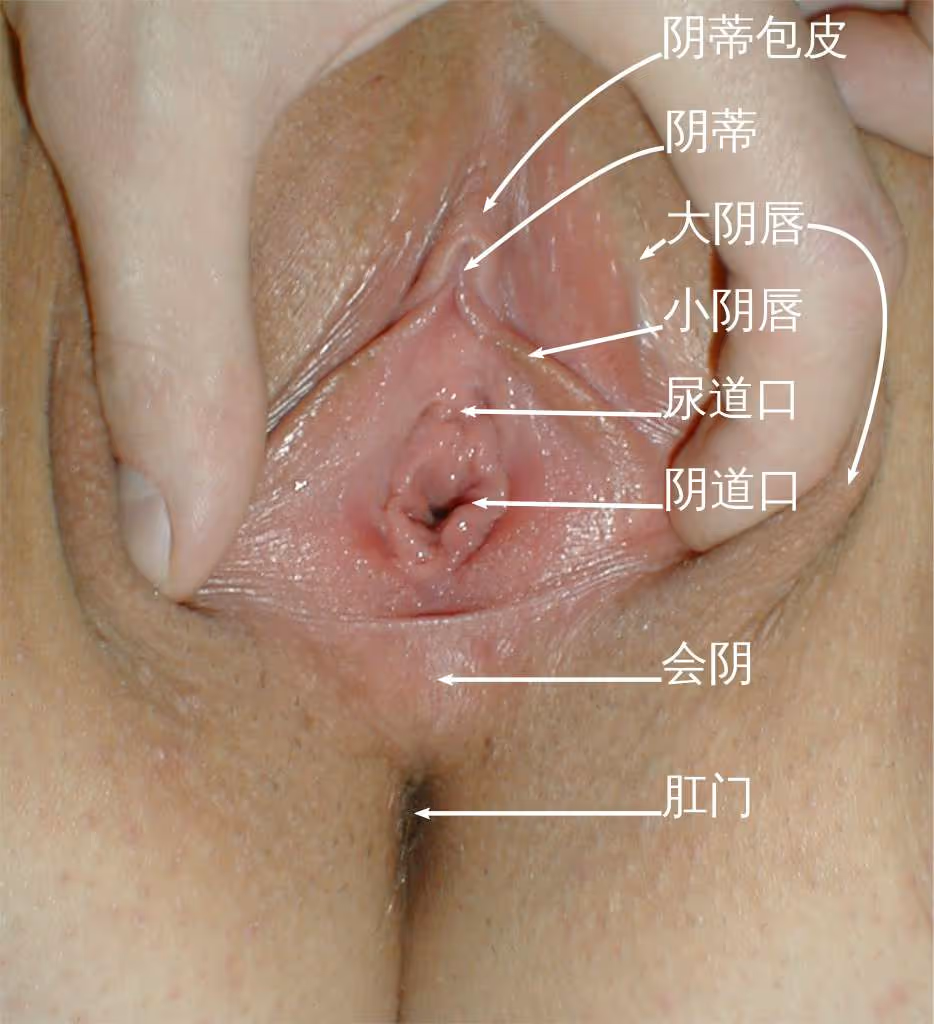
\includegraphics[width=0.7\linewidth]{Images/1}
	\caption{}
	\label{fig:1}
\end{figure}

\begin{figure}
	\centering
	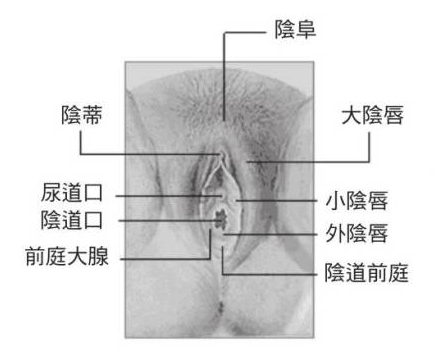
\includegraphics[width=0.7\linewidth]{Images/2}
	\caption{}
	\label{fig:1}
\end{figure}

\subsection{内生殖器官}

卵巢呈卵圓形,位於盆腔內子宮的兩側,左右各一。卵巢發育成熟後,能產生成熟的卵子,並分泌雌性激素,維持女性特徵。在一個月經週期中,卵巢內常有幾個甚至十幾個卵泡同時發育,但一般只有一個發育成卵子。

輸卵管位於子宮兩側,是輸送卵子進入子宮的彎曲管道。輸卵管内端與子宮腔相通,外端游離。輸卵管管壁由黏膜、肌層及外膜三層組成。黏膜上皮為單層柱狀纖毛上皮。纖毛具有擺動功能。肌層的蠕動及纖毛的擺動,有助於受精卵進入子宮腔内。

子宫位於骨盆腔内,在膀胱與直腸之間,形狀似倒置的梨子,前後略扁,分宮底、宮體、宮頸三部分,上通輸卵管,下接陰道。

子宫是孕育胎兒的器官,又是產生月經的場所。子宮壁共分三層,由外向內為外膜、肌層和内膜。

陰道是一種收縮性很強的肌性管道,上通子宮頸管,下開口於陰道前庭,陰道前壁緊貼膀胱和尿道,後壁與直腸相鄰。陰道為性交器官,又是月經排出和胎兒娩出的通道。

\begin{figure}
	\centering
	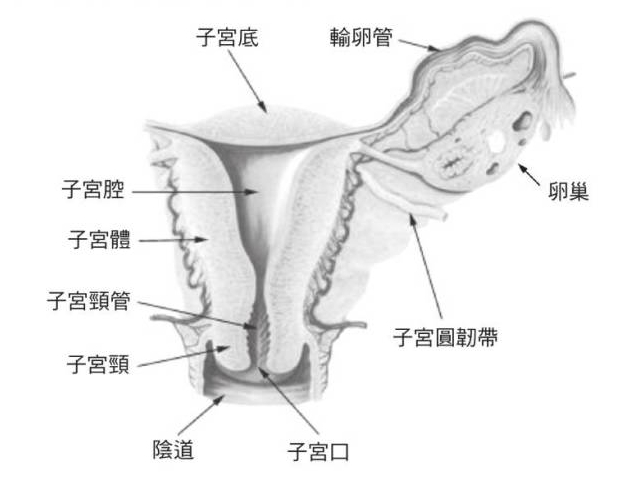
\includegraphics[width=0.7\linewidth]{Images/3}
	\caption{}
\end{figure}

\section{男性生殖器官}

男性生殖器官分為外生殖器官和内生殖器官兩部分。外生殖器包括陰阜、陰囊和陰莖,而內生殖器由睾丸、附睾、精索、輸精管及射精管、精囊腺、前列腺、尿道球腺、尿道等組成。

\subsection{外生殖器官}

陰阜為恥骨前方的皮膚和豐富的皮下脂肪組織。青壯年時陰阜顯著隆起,中年以後脂肪組織減少下陷,老年則萎縮變平。

陰囊是由皮膚、肌肉等構成的柔軟而富有彈性的袋狀囊,裏面有睾丸、附睾、精索,主要功能有保護睾丸、調節溫度、有利於精子的產生和貯存等。陰囊內有陰囊隔,将陰囊內腔分成左右兩部分,各容納一個睾丸和附睾。陰囊皮膚薄而柔軟,並有很多的褶皺。陰囊皮膚有明顯的色素沉著,长有稀疏的陰毛。

\begin{figure}
	\centering
	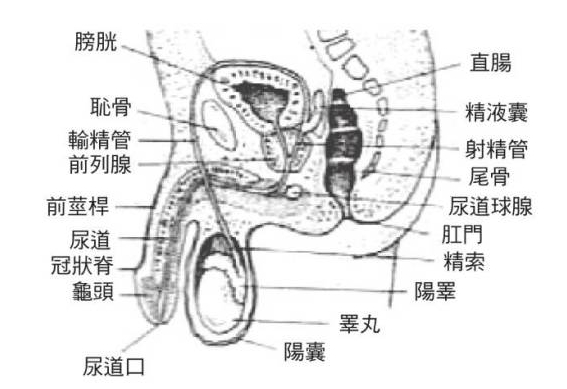
\includegraphics[width=0.7\linewidth]{Images/4}
	\caption{}
\end{figure}

陰莖後部為陰莖根,中部為呈圓柱形的陰莖體,其前端膨大部分為陰莖頭(俗稱「龜頭」)。陰莖軸與陰莖頭之間是冠狀溝,陰莖頭與冠狀溝含有豐富的神經末梢,對刺激是很敏感的,而冠狀溝處神經分佈最豐富,敏感性最高。陰莖體由陰莖海綿體和尿道海綿體組成,具有豐富的血管、神經、淋巴管。從外形上看,陰莖有鬆弛和勃起兩種狀態,具有排尿、性交、射精三大功能。

\subsection{内生殖器官}

睾丸是男性生殖腺,呈卵圆形,左右各一,由精索将其懸吊於陰囊內,长約4~5公分,厚約3~4公分,約重15公克左右。睾丸是產生雄性生殖細胞(即精子)的器官,也是產生雄性激素的主要内分泌腺體。

附睾位於睾丸的後外側,外形細长,似半月形,左右各一,长約5公分。附睾有儲存和排放精子、促使精子成熟及供給精子營養的作用。

精索位於睾丸上端至腹股溝管腹環之間,左右各一,全长約14公分。精索是睾丸、附睾及輸精管血液、淋巴液循環的通路,也是保證睾丸的生精功能及成熟精子輸送的主要途徑。輸精管是精索內的主要結構之一,其末端與精囊腺的排泄管匯合成射精管,穿過前列腺,開口於尿道,全长約40~46公分,直徑約2~3公釐。

輸精管是精子從附睾被輸送到前列腺部尿道的唯一通路。射精管是輸精管壺腹與精囊管匯合之後的延續。射精管很短,长僅為2公分左右,管壁很薄。

精囊腺為一對扁平长囊狀腺體,左右各一,表面凹凸不平呈結節狀,其末端細小為精囊腺的排泄管,與輸精管的末端匯合成射精管,在尿道前列腺部開口於尿道。精囊长4~5公分,寬約 2公分,容積約4C.C。精囊為屈曲狀的腺囊,其分泌液主要為精漿液,占精液的70\%左右,對精子的存活有重要作用。前列腺為一個栗子狀的腺體,平均重量約20公克,是男性最大的附属腺體,能分泌前列腺液,組成精漿液。前列腺還被認為是一個性敏感部位,對其進行適當刺激時,可以引起性興奮。尿道球腺左右各一,位於尿道生殖隔上下筋膜之間的會陰深囊內,開口於球部尿道近端,可分泌少量液體,為精漿的成分之一。

男性尿道长12~20公分,既有排尿功能,又有排精的功能。

其中有尿道球腺,可分泌液體,參與精液的組成,性交時有潤滑陰莖頭的作用。

\chapter{性慾}

簡單地說,性慾就是對性生活的一種慾望,它既受體內激素水準的調節,也受社會、家庭等周圍環境因素的影響。同時存在比較大的個體差異,即使是同一個人,性慾的高低也隨年齡、心理狀態、患病狀況、生活品質、工作環境、婚姻狀態等不同而表現不同。

一般情况下,性慾源於性心理的驅動,比如對異性的愛慕可以誘發性慾。男女之間建立美滿家庭以及夫妻間的親暱,都會產生性交的慾望。性慾產生的另外一個原因與內分泌有關。青春期過後,驟然提高的人體性激素分泌水準會驅動性慾。男性精囊、前列腺等性腺内分泌物的增加與淤積,女子外陰前庭大腺等分泌物的過多貯存,都可誘發性刺激和促進性慾。此外,既往性生活的愉快感受,或者男女之間身體接觸產生的性刺激等,也可以誘發性慾。所以,性慾是多方面因素綜合作用的結果,不但思維、意識、情感、環境等因素與性慾相關,而且語言、文字、圖畫、音樂等,也會給性慾帶來舉足輕重的影響。

男人的性慾和女人的性慾一樣嗎

從表面上看,男人的性慾似乎比女人強,因為在性生活中居於主動地位的女性比較少,這裏面既有生理上的因素,但主要還是心理因素的影響。許多女人習慣於壓抑自己的性需求,所以,在多數情況下,男人的性慾表現得比女性主動,但這不證明男人的性慾就比女人的性慾強。

處於青春期的男性比女人更富於性幻想,並容易將感情需要和性需要混為一談。成年以後,工作的壓力和家庭的負擔,會使青春期旺盛的性渴望減弱,但仍有少數人性慾一直比較強烈,在這一點上,女人和男人是一樣的。男性的性慾在某些年齡階段表現得要比女人強,但在另一些年齡階段卻可能完全相反。在性生活不和諧的夫妻中,產生性慾低下的一方往往是丈夫,其中年齡是個重要因素,男人的性慾高潮期通常在30歲以前,而女人則是在40歲左右,才對性活動表現出濃厚的興趣。

為什麼有的人性慾強,有的人性慾弱

性慾是有很大的個體差異的。性慾的強弱程度與下列因素有關:

①遺傳因素:性慾的強弱程度受遺傳因素的影響,一個家族的成員,往往表現出類似的性慾傾向。

②激素水準:人體中有多種激素,男女皆然。在多種激素中,雄性激素對性慾的影響最大。雄性激素水準高,性慾就強,雄性激素水準低,性慾就弱,無論男女都一樣。

③感覺刺激:在多種刺激下,人體就會產生各種各樣的感覺,如視覺、味覺、聽覺、嗅覺、觸覺等,這些感覺可以激起性慾,在這一點上男性和女性沒有明顯差異。

④性體驗和性經驗:如果以往性體驗順利並且性經驗豐富,性喚起就比較容易;反之,性慾的產生就比較困難。

⑤環境因素:人體會對外界環境的刺激作出多種反應,所以生活環境中的光照、溫度、濕度、季節、飲食等因素,都會影響性慾的產生。

⑥文化因素:性慾的產生是一種個人行為,但性慾也與文化因素有關,在某種程度上它必須接受倫理、法律、道德,甚至醫學的約束。

⑦情緒變化:心理狀態影響著性慾的產生,比如當人們被憂慮、恐懼、憤怒、抑鬱、疼痛、痛苦所困擾的時候,一般是很難產生性慾的。

⑧年齡因素:人的性慾會隨著年齡的變化而變化。就一般規律而言,男性的性慾高峰在30歲之前,而女性則是在40歲以後性慾最為高漲。隨著年齡的增加、内分泌的改變,體內雄性激素的減少,人體感覺會變得遲鈍,導致性器官血液循環不良,再加上來自事業、生活及社會交往等方面的壓力,這些因素都會使人的性慾減
退。

⑨健康因素:健康的生理狀態是維持性慾的基礎。人體的各種疾病,如内分泌、生殖器官、代謝系統、腫瘤及其他消耗性疾病,都會影響性慾的產生。

總之,性慾是人的生理本能之一,它受多種因素的影響。

不要將性慾望和性功能混為一談

現實生活中,不少人對性都存在認識上的誤區,將性慾望和性
功能混為一談即是其中之一。實際上,這兩者還是有區別的。
所謂性慾望是對性的一種要求、一種渴望的心情,而性功能則
是將慾望化做具體行為的能力,完美和諧的性生活,需要性慾望和
性功能的協調和統一。如果能將性慾望和性功能協調於一身,就能
充分享受性所帶給自己的愉悅;但是要想實現這個願望,需要不斷
地摸索和探尋,如果沒有完成這種轉化,就會導致性的各種不和諧
和性功能障礙。
實際上,性慾望和性功能分離的情況是很常見的,常見原因有
生理性的,也有精神心理性的,還有疾病等因素。比如,進入青春
期的青少年,開始出現朦朧的性意識,也具有了陰莖勃起的能力,
但他們對性的慾望還沒有建立起一個明確的概念;一個習慣自慰的
青年,有可能擔心自己患了陽痿,懷疑自己的性能力;老年男性,
儘管歲月的磨煉使他們更加珍愛生活、珍愛愛情,對於性的要求
(慾望)也很高,但是性功能卻在慢慢地減退,直至消失;患有某
些疾病的男子,儘管主觀上很想「要」,但實際能力卻不行;某些

傳染病患者,儘管性功能很好,但為了疾病的康復,必須抑制自己
的性慾望。



\backmatter

\end{document}